\documentclass{beamer}
%Information to be included in the title page:
\title{Comparison of amplifiers}
\author{Paul Deguire}
\institute{Interview Multimessenger School}
\date{January 2024}

\begin{document}

\frame{\titlepage}

\begin{frame}
\frametitle{}
\begin{figure}
    \centering
    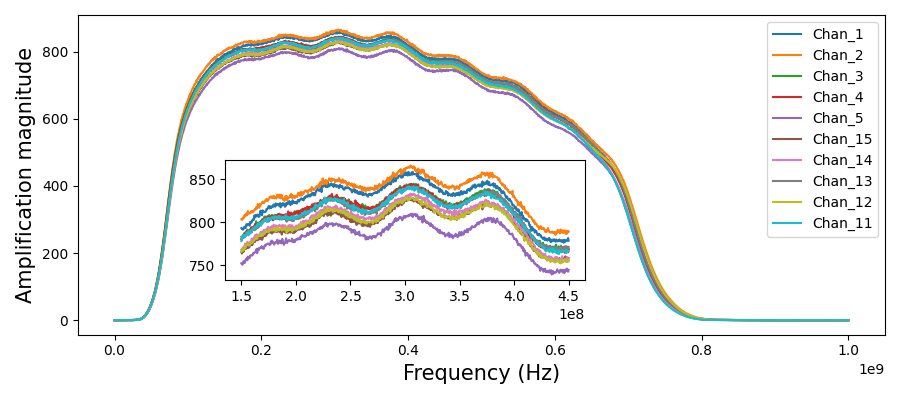
\includegraphics[width=0.9\textwidth]{../figures/all_amp.png}
    %\caption{Caption}
    %\label{fig:enter-label}
\end{figure}
\begin{itemize}
    \item We observe the same patterns for all amplifiers. The signal is amplified for frequencies between $\sim100$ MHz and $\sim650$ MHz with a maximum of amplification of $\sim800$.
    \item For frequencies in this bandwidth, the amplifier Chan\_5 (purple) is the one with the lowest amplification and the amplifier Chan\_2 (orange) is the one with the highest amplification.
\end{itemize}
\end{frame}

\begin{frame}
\frametitle{}
\begin{columns}
\begin{column}{0.5\textwidth}
\begin{figure}
    \centering
    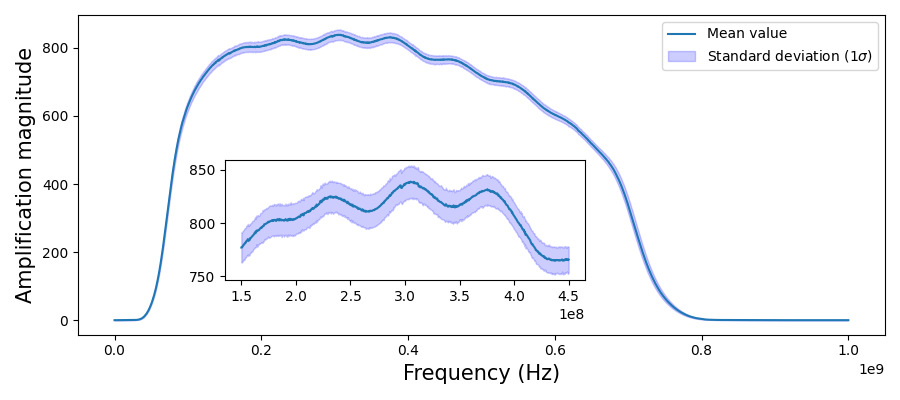
\includegraphics[width=\textwidth]{../figures/uncert.png}
    %\caption{Caption}
    %\label{fig:enter-label}
\end{figure}
\begin{figure}
    \centering
    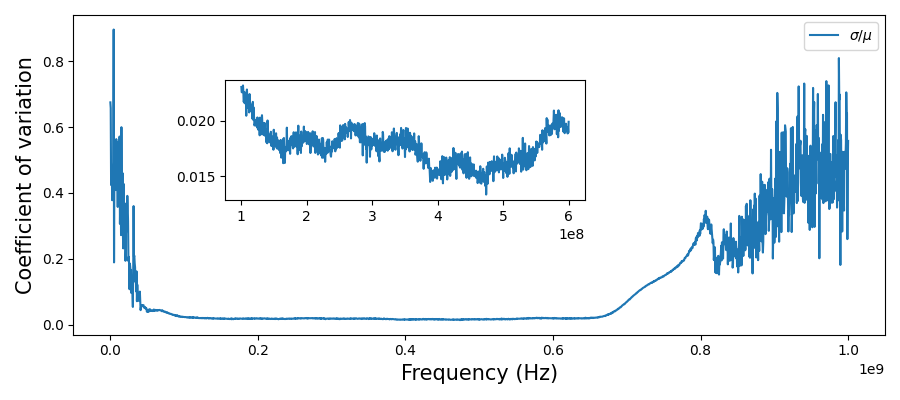
\includegraphics[width=\textwidth]{../figures/cv.png}
    %\caption{Caption}
    %\label{fig:enter-label}
\end{figure}
\end{column}
\begin{column}{0.5\textwidth}
    \begin{itemize}
        \item We assume all amplifiers should have the same characteristics. The top figure shows the mean value and the uncertainty as a function of the frequency.
        \item Amplifiers amplify the signal (they reach at least 50\% of the maximum amplification) between $78.4\pm0.6$ MHz and $685\pm4$ MHz.
        \item The coefficient of variation ($\sigma/\mu$) is the lowest for this interval (see bottom figure).
    \end{itemize}
\end{column}
\end{columns}
\end{frame}


\end{document}
